% Chapter Template

\chapter{Phase 1 - Investigation} % Main chapter title

\label{Chapter4} % Change X to a consecutive number; for referencing this chapter elsewhere, use \ref{ChapterX}

%----------------------------------------------------------------------------------------
%	SECTION 1
%----------------------------------------------------------------------------------------
The aim of the investigation phase is to obtain a more nuanced understanding regarding the differences in perception and navigation of western versus Chinese websites. This information will facilitate the decision making process concerning which features to keep, which features need to be analysed, and what usability metrics should be implemented in the study. 

\section{Work process}
As an initial step, Chinese websites a long with their western equivalents were identified and curated. After obtaining a corpus of websites from China and western countries (e.g., United Kingdom), the key design differences between these respective sites were documented. Once the primary design variances were explored, this information was used to decide which design patterns should be tested in the study. Finally, the specific metrics to measure the results of these different designs were concluded. 


\section{Chinese vs Western websites comparison}
In reviewing the websites, it was evident that Chinese pages differed significantly from western  counterparts. The differences between sites extend from the look and feel to the UX design. A few of China's most popular browsing sites will be analysed and compared to similar western counterparts to further investigate these design distinctions. 
 
\subsection{BBC}
BBC is a very popular western new site. The design is quite westerly influenced in terms of information density and design. As can be seen in the fig... the site follows the f-shaped pattern quite heavily. Each news section has a large news figure in the top left corner and two rows. Just looking at the large picture and the first row then glazing down to the next news section would have the users quite naturally follow the f-shaped pattern (fig med röd färg). The site itself is quite information sparse with large images taking most of the space. Without hovering over any content on a standard computer screen, there are roughly 48 clickable elements.

\subsection{QQ}
QQ is one of the  most visited websites in China (see fig \ref{fig:QQ.com}). \cite{top_sites_china} \cite{top_sites_alexa} QQ, like many other Chinese websites, does not focus on one thing but has multiple different functions. Some of the functions that QQ supports are: instant messaging, online  games, music, shopping, microblogging, news, movies, group chat software, and etc. On the QQ homepage, users are greeted by the site's news page, which is highly information dense. Without hoovering over any content on a standard computer screen, there are roughly 147 clickable elements.  In contrast,  BBC's homepage \cite{bbc}, which is considered fairly information dense by western standards, has only 48 clickable elements on its homepage. This means that with only counting clickable elements, QQ is over 3 times more information dense than BBC. 


\begin{figure}[h]
\centering
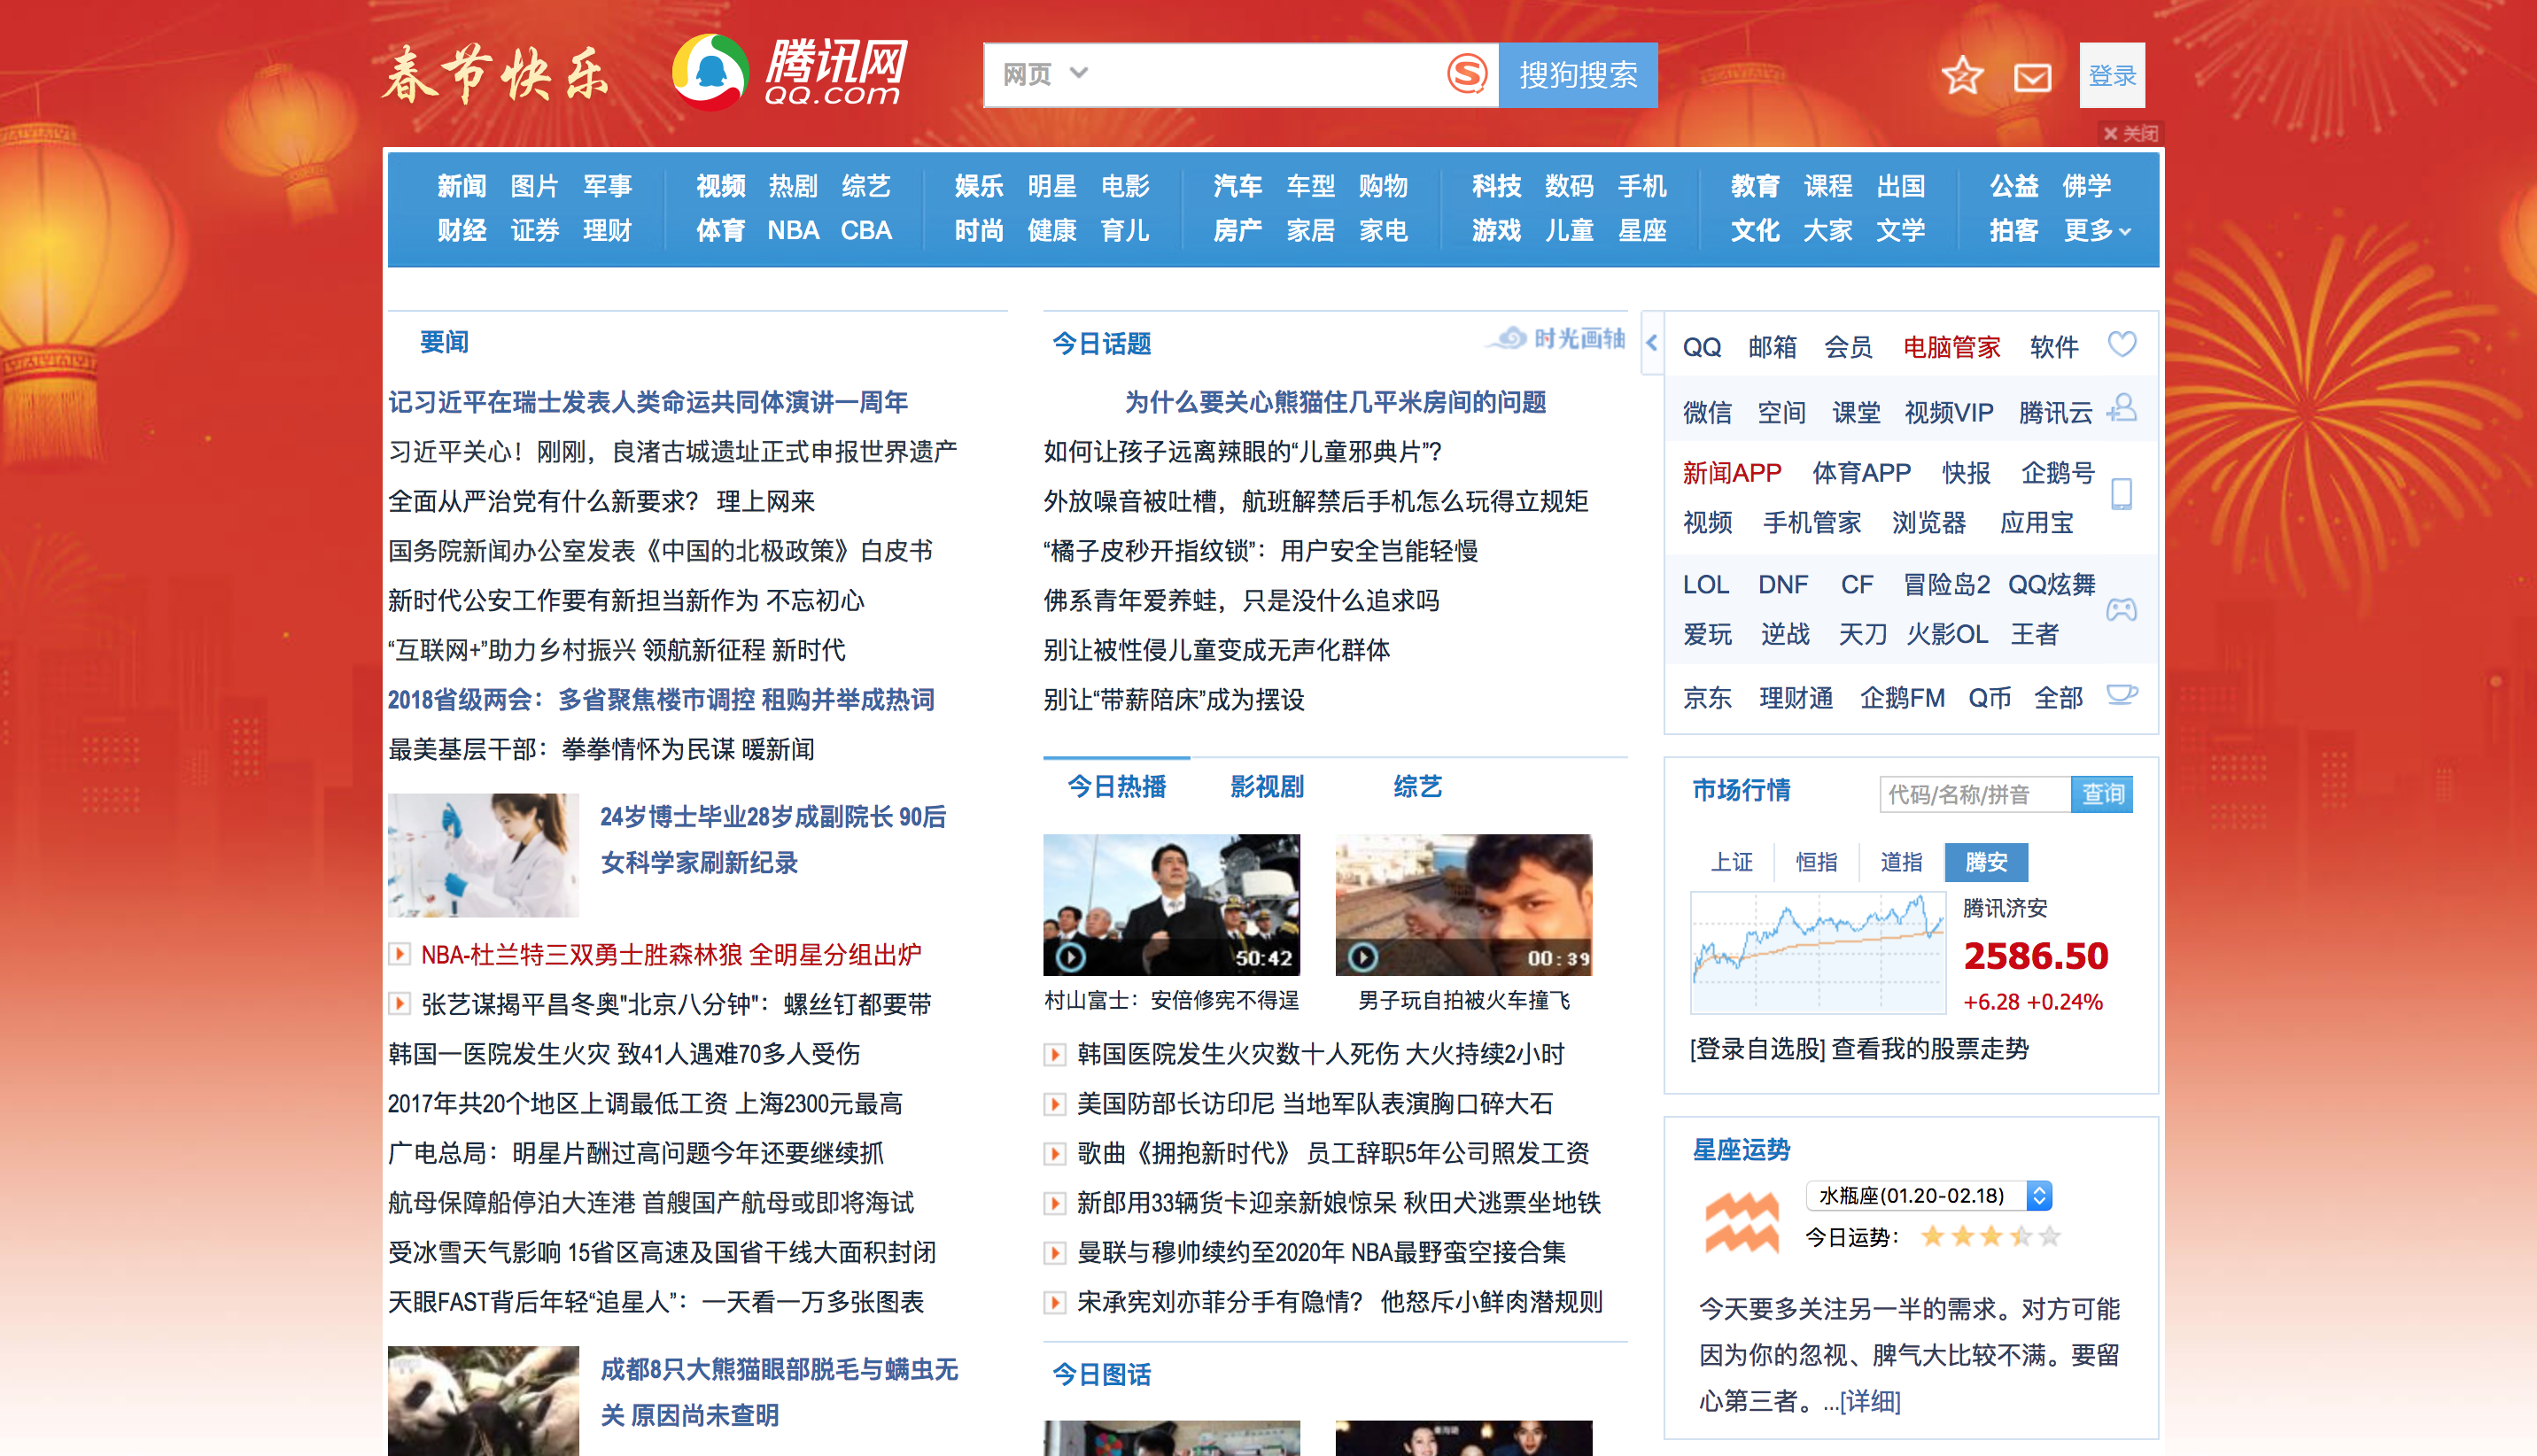
\includegraphics[width=100mm]{Images/QQ.png}
\decoRule
\caption[QQ.com]{QQ's homepage which provide which is mostly used for news.}
\label{fig:QQ.com}
\end{figure}
One element that is notably common on Chinese websites, including QQ, is the menu bar design (see fig \ref{fig:QQ_menubar}). On the QQ page, the menu bar contains two rows with a total of 40 clickable options - this format of menus is typical in China and is shared by multiple  other Chinese sites. 


\begin{figure}[h]
\centering
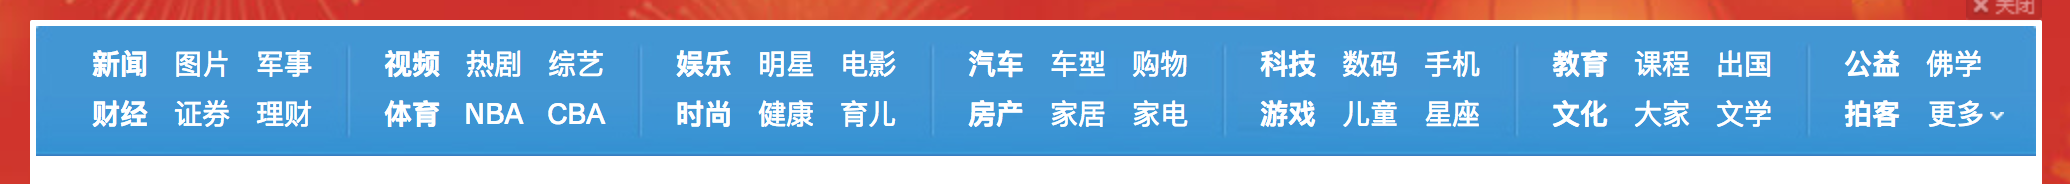
\includegraphics[width=100mm]{Images/QQ_menubar.png}
\decoRule
\caption[QQ's Menu bar]{A close-up of the menu bar used at QQ.}
\label{fig:QQ_menubar}
\end{figure}



\subsection{Taobao and Ebay}
Taobao, which provides services akin to America's Ebay, is one of the world's biggest e-commerce platforms. Both Taobao and Ebay are shopping websites where users can purchase nearly any product they need, both from retailers and from other consumers. However, although these sites are similar in service, the design and user-experience focus on these sites differ significantly. Ebay, for instance, boasts a sleek design, employing dark-themed colors and contains only 20 clickable elements on the home page (see fig:\ref{fig:ebay}). Conversely, the Taobao page contains more colors, employs a brighter theme, and incorporates more clickable elements compared to its western counterpart. Another notable distinction between the websites is that Ebay has an expanding menu bar containing roughly 6-10 clickable elements while Taobao's menu contains much more (see fig:\ref{fig:ebay_menu}).

\begin{figure}[h]
\centering
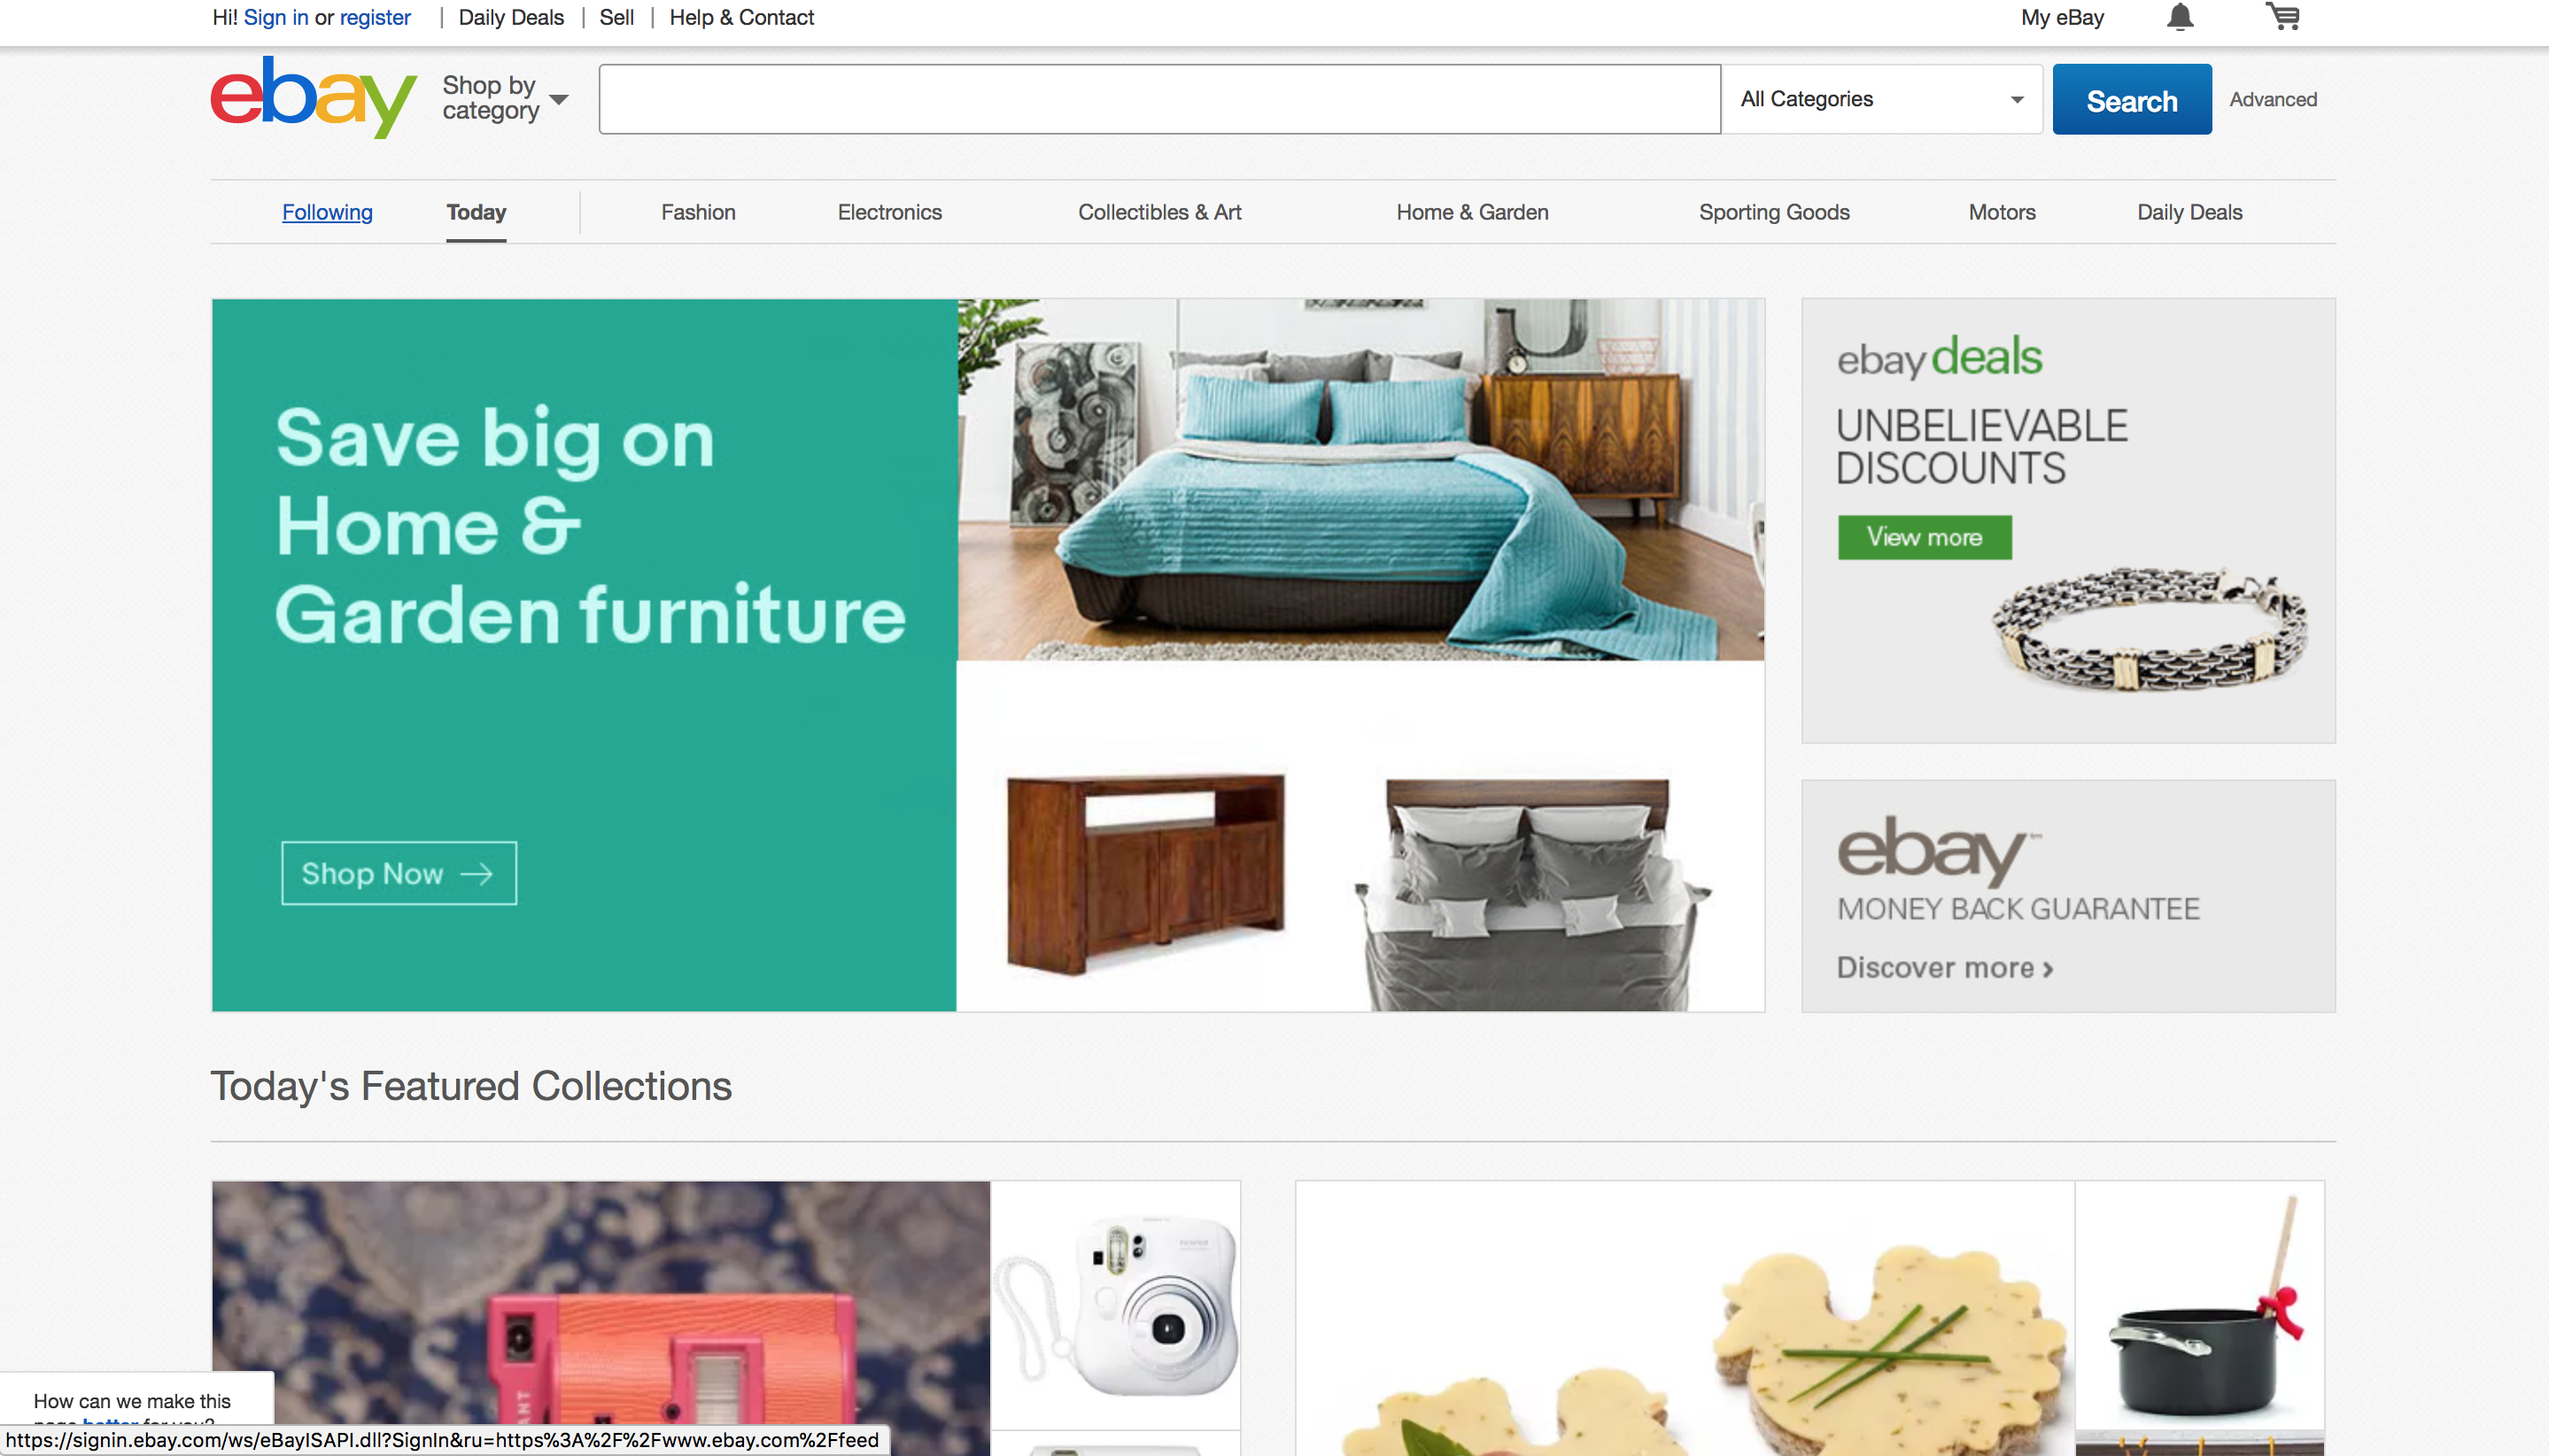
\includegraphics[width=100mm]{Images/ebay.png}
\decoRule
\caption[ebay]{Ebay a popular American online shopping site}
\label{fig:ebay}
\end{figure}

\begin{figure}[h]
\centering
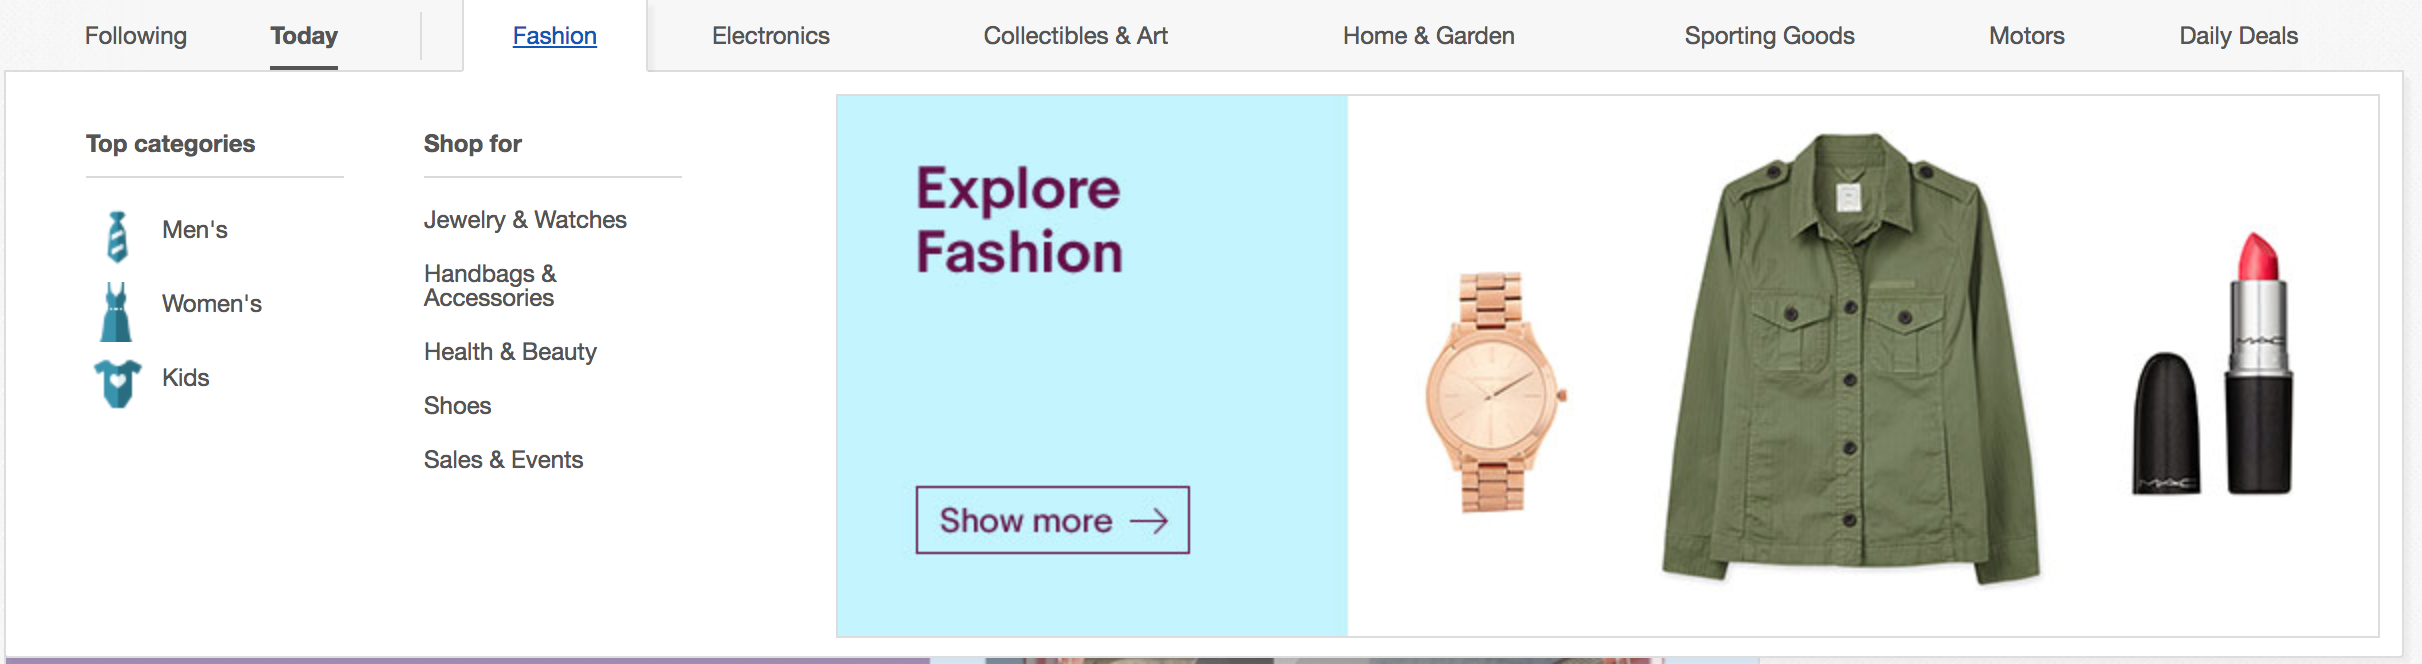
\includegraphics[width=100mm]{Images/ebay_menu.png}
\decoRule
\caption[Ebay's menu bar]{Expanding the menu on Ebay.}
\label{fig:ebay_menu}
\end{figure}

In examining the Chinese version of Taobao, the difference in information density is evident (see fig:\ref{fig:taobao}). The main page, for example, hosts roughly 49 clickable elements. Additionally, the menu items on the screen's right side is expandable, displaying between 55 to 88 clickable links and elements see fig:\ref{fig:taobao_menu}). This amounts to about eight times the amount of clickable elements on Ebay. Further, while Taobao employs strong color themes (e.g., red, purple, orange, and blue), Ebay generally employs muted colors (e.g., grey) allowing for the products to be the center of focus. 


\begin{figure}[h]
\centering
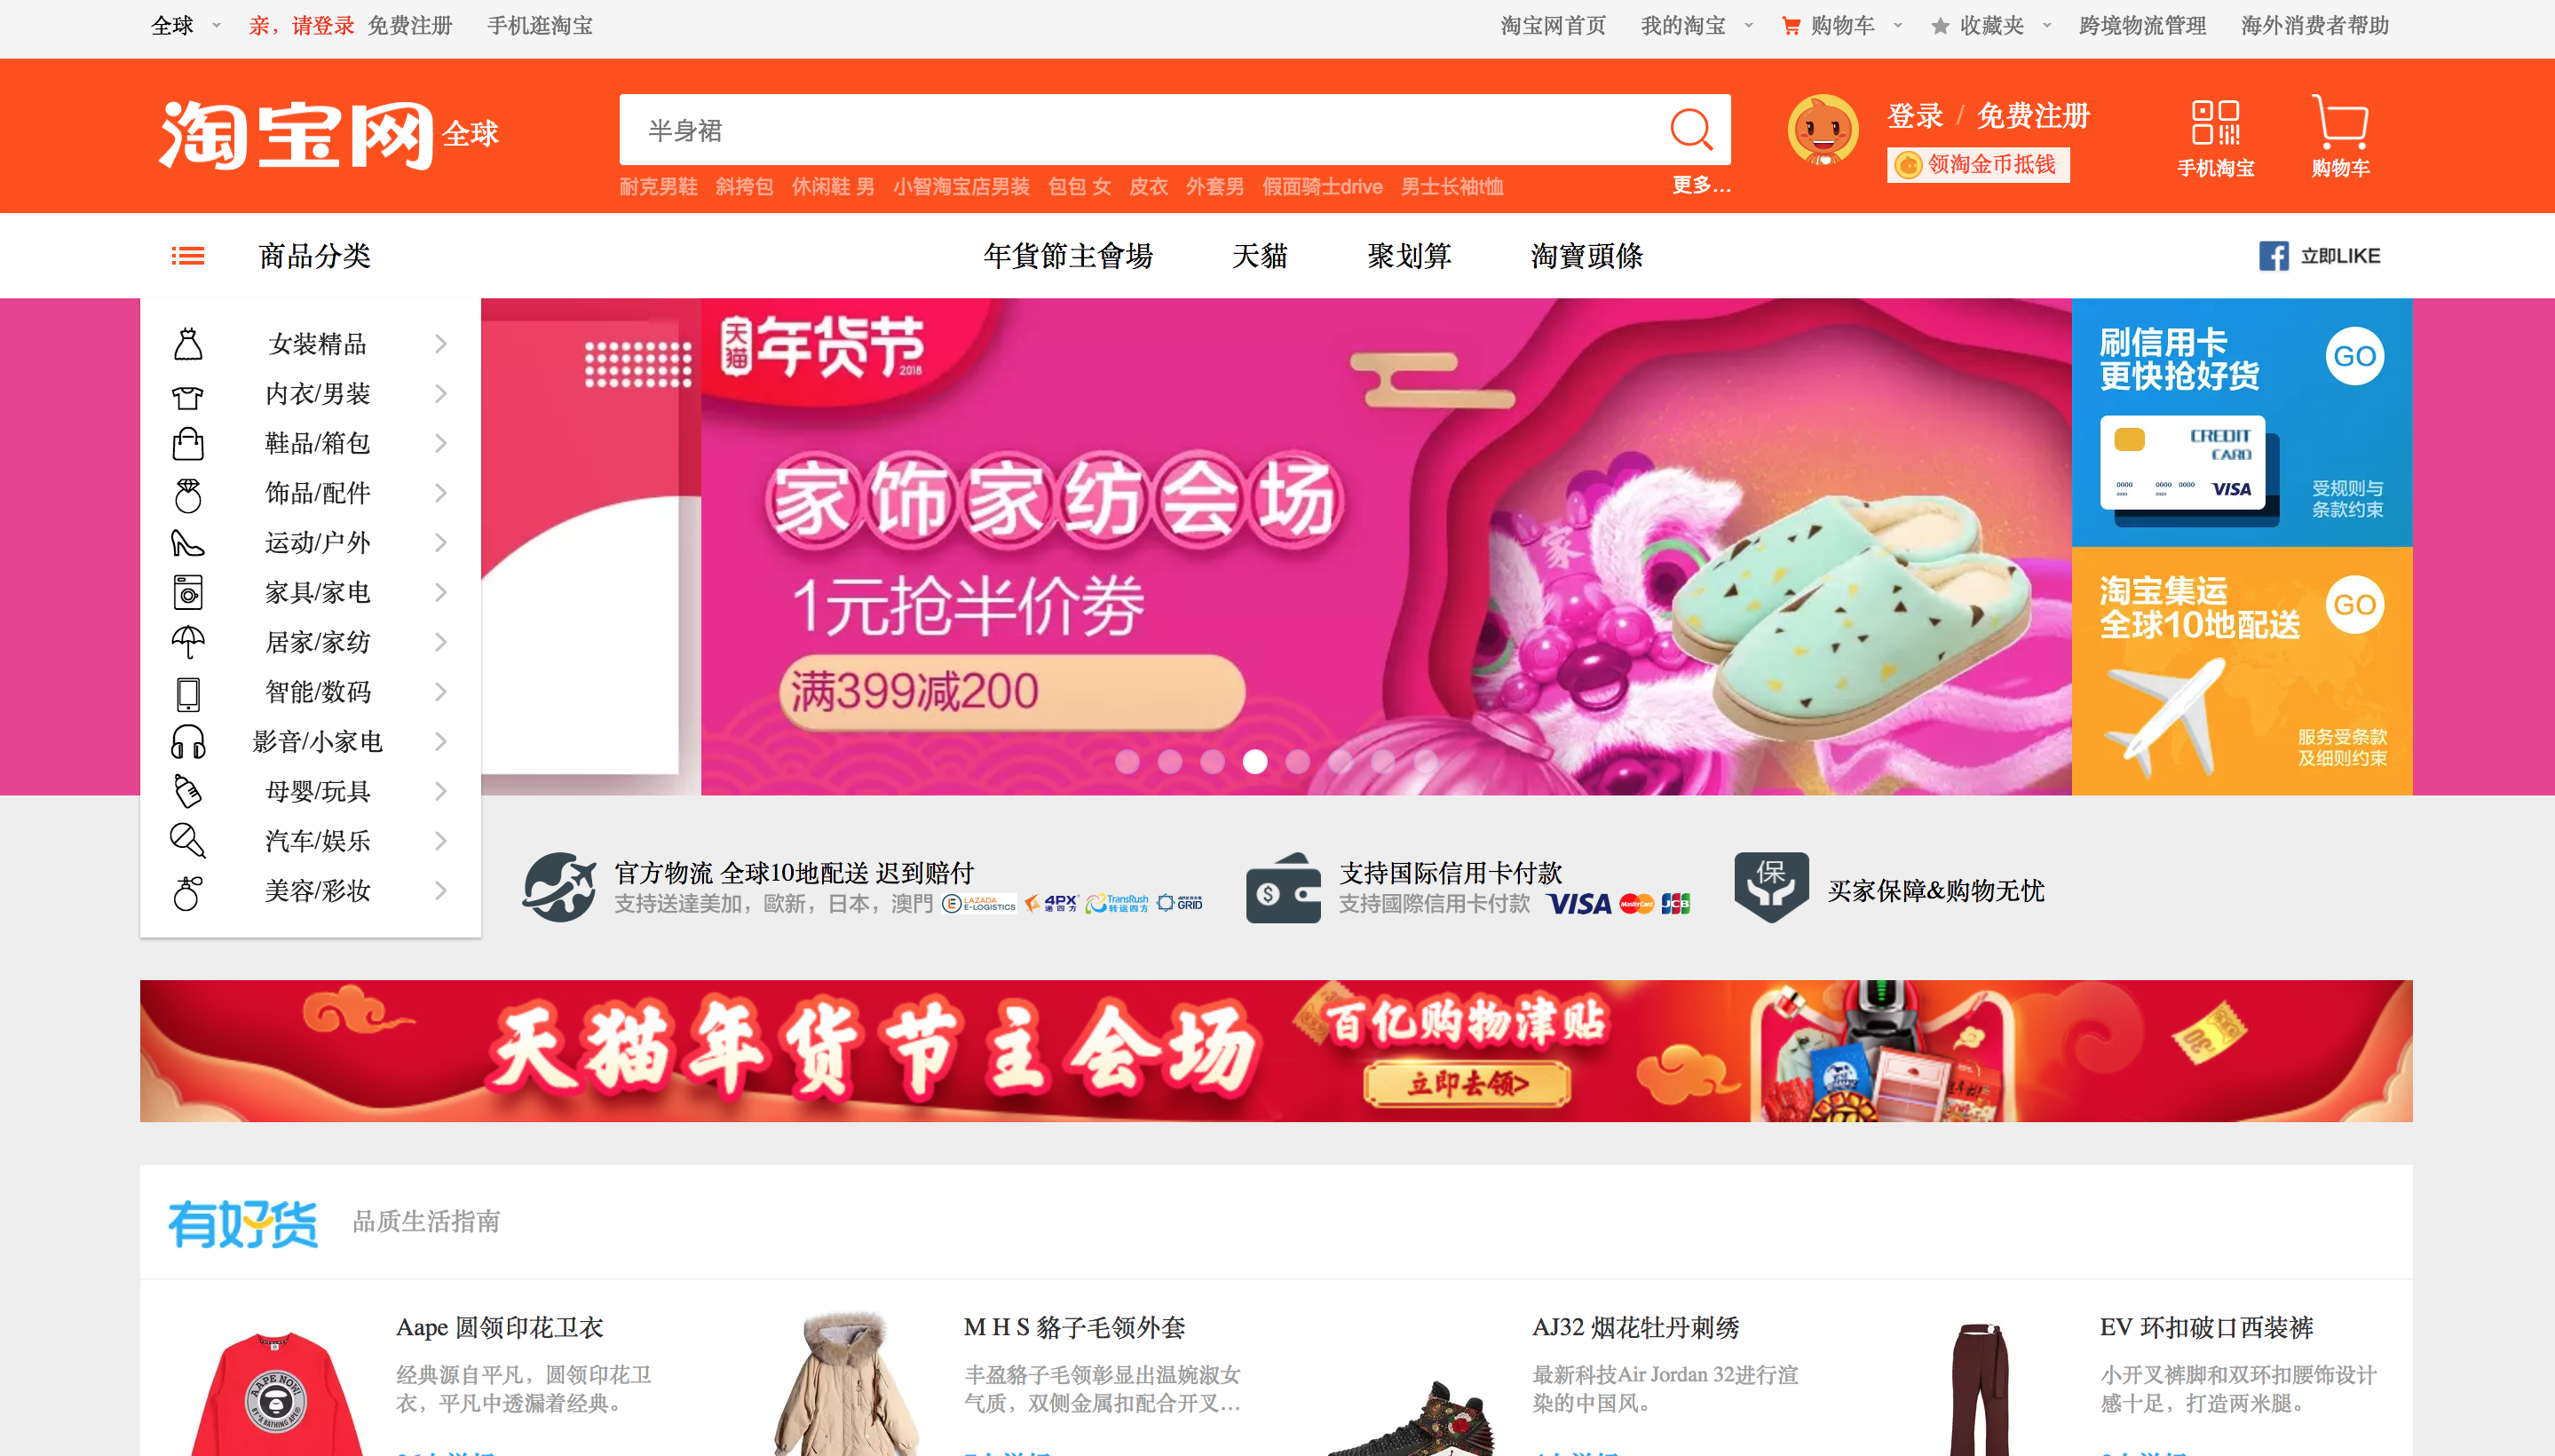
\includegraphics[width=100mm]{Images/Taobao}
\decoRule
\caption[Taobao]{Taobao a popular Chinese online shopping site}
\label{fig:taobao}
\end{figure}

\begin{figure}[h]
\centering
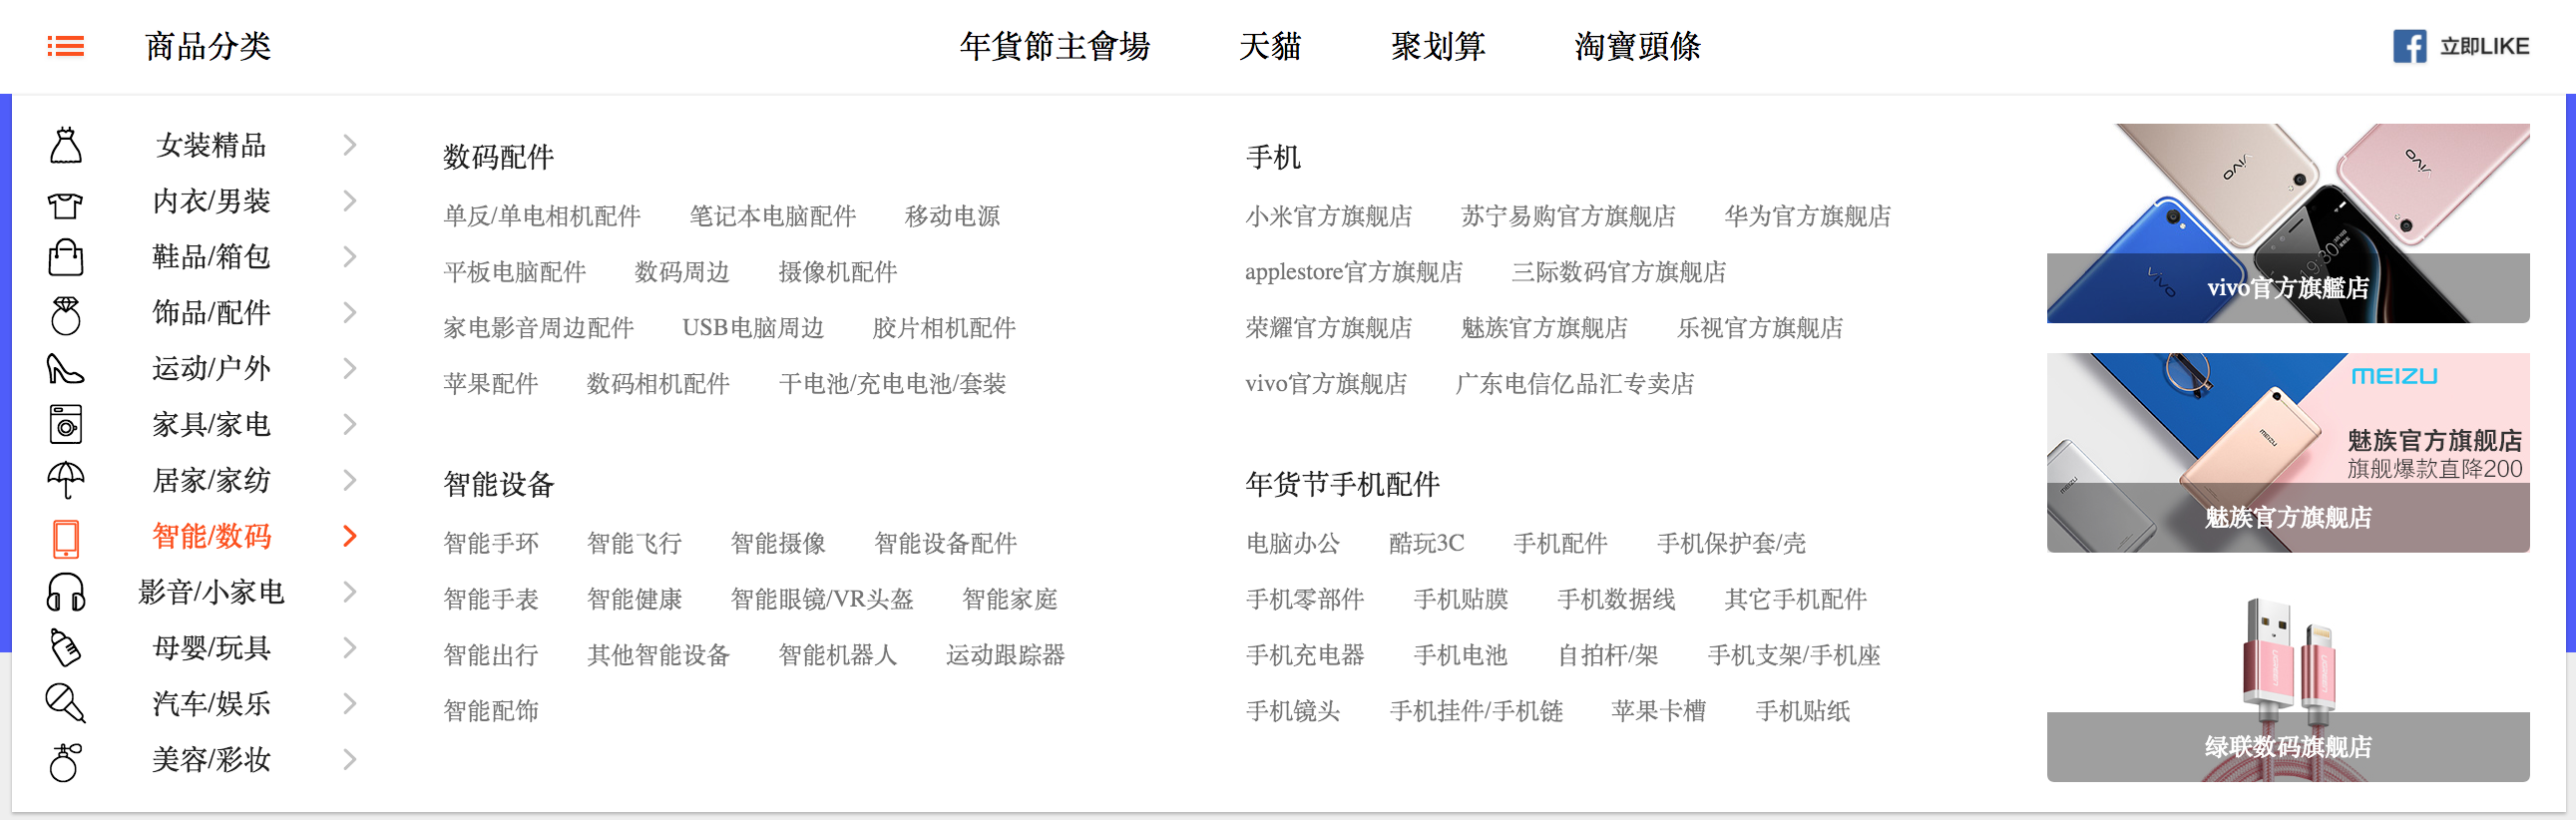
\includegraphics[width=100mm]{Images/Taobao_menu}
\decoRule
\caption[Taobao' menu bar]{Expanding the menu on Taobao.}
\label{fig:taobao_menu}
\end{figure}

\subsection{Analyses of Ctrip}
Interestingly, the layout on many Chinese websites change significantly when the language is changed. For instance, the layout of Ctrip, a common travel site used for booking hotels and flights in China, becomes very different when users select English for the site (see  fig: \ref{fig:ctrip_chinese} versus for the Chinese version (see fig: \ref{fig:ctrip_english} for English version). With the exception of the brand and name of the website, it is difficult to tell that it is actually the same website .

\begin{figure}[h]
\centering
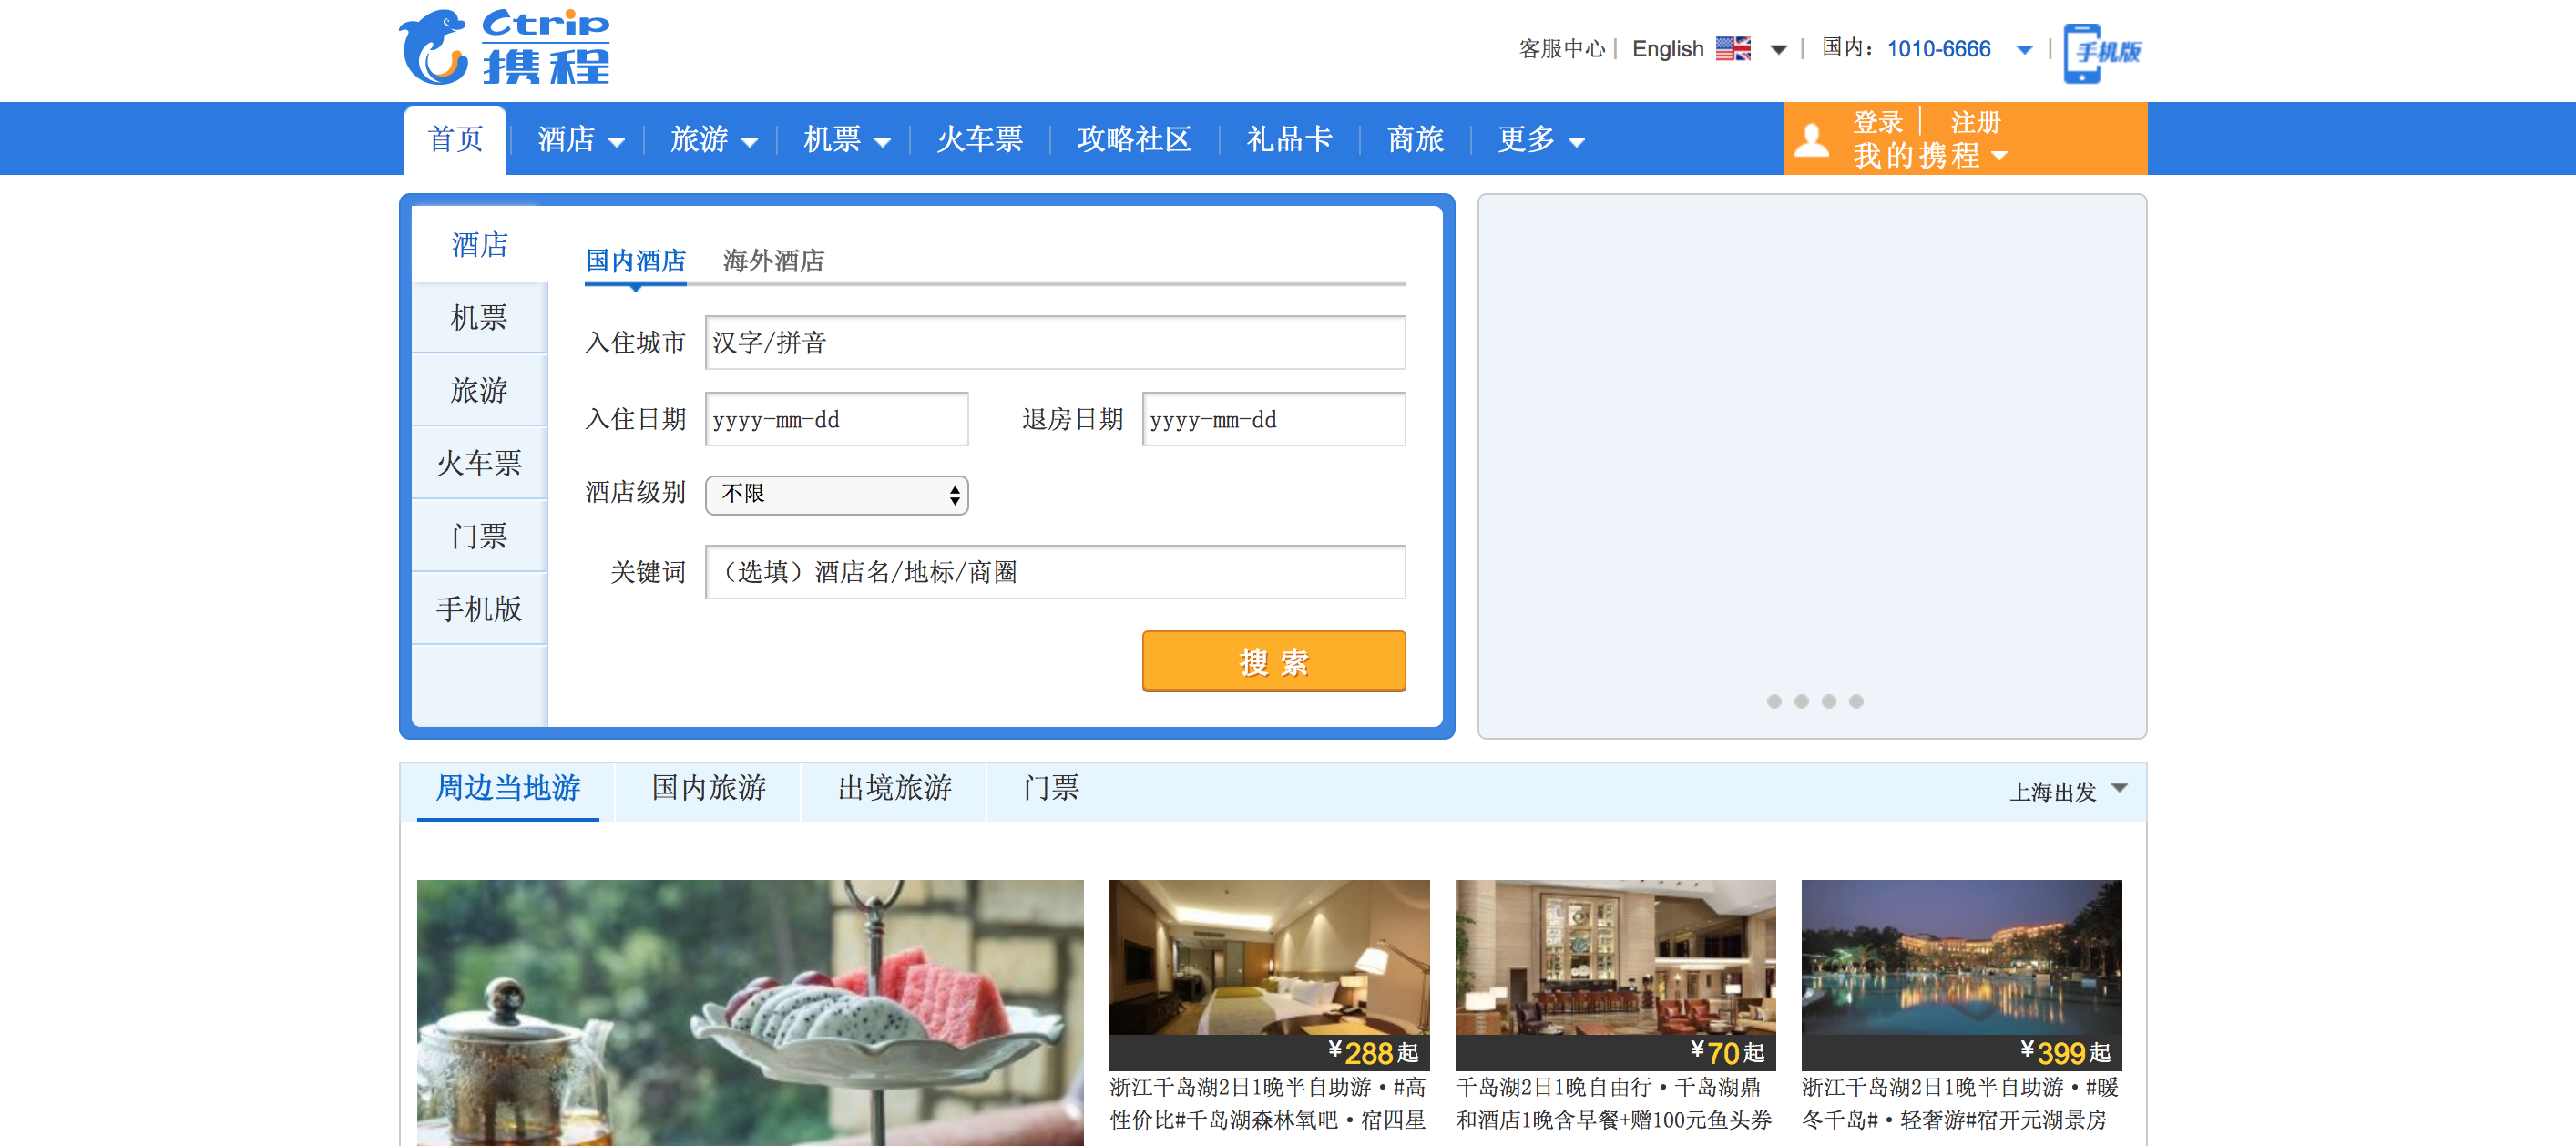
\includegraphics[width=100mm]{Images/ctrip_chinese1}
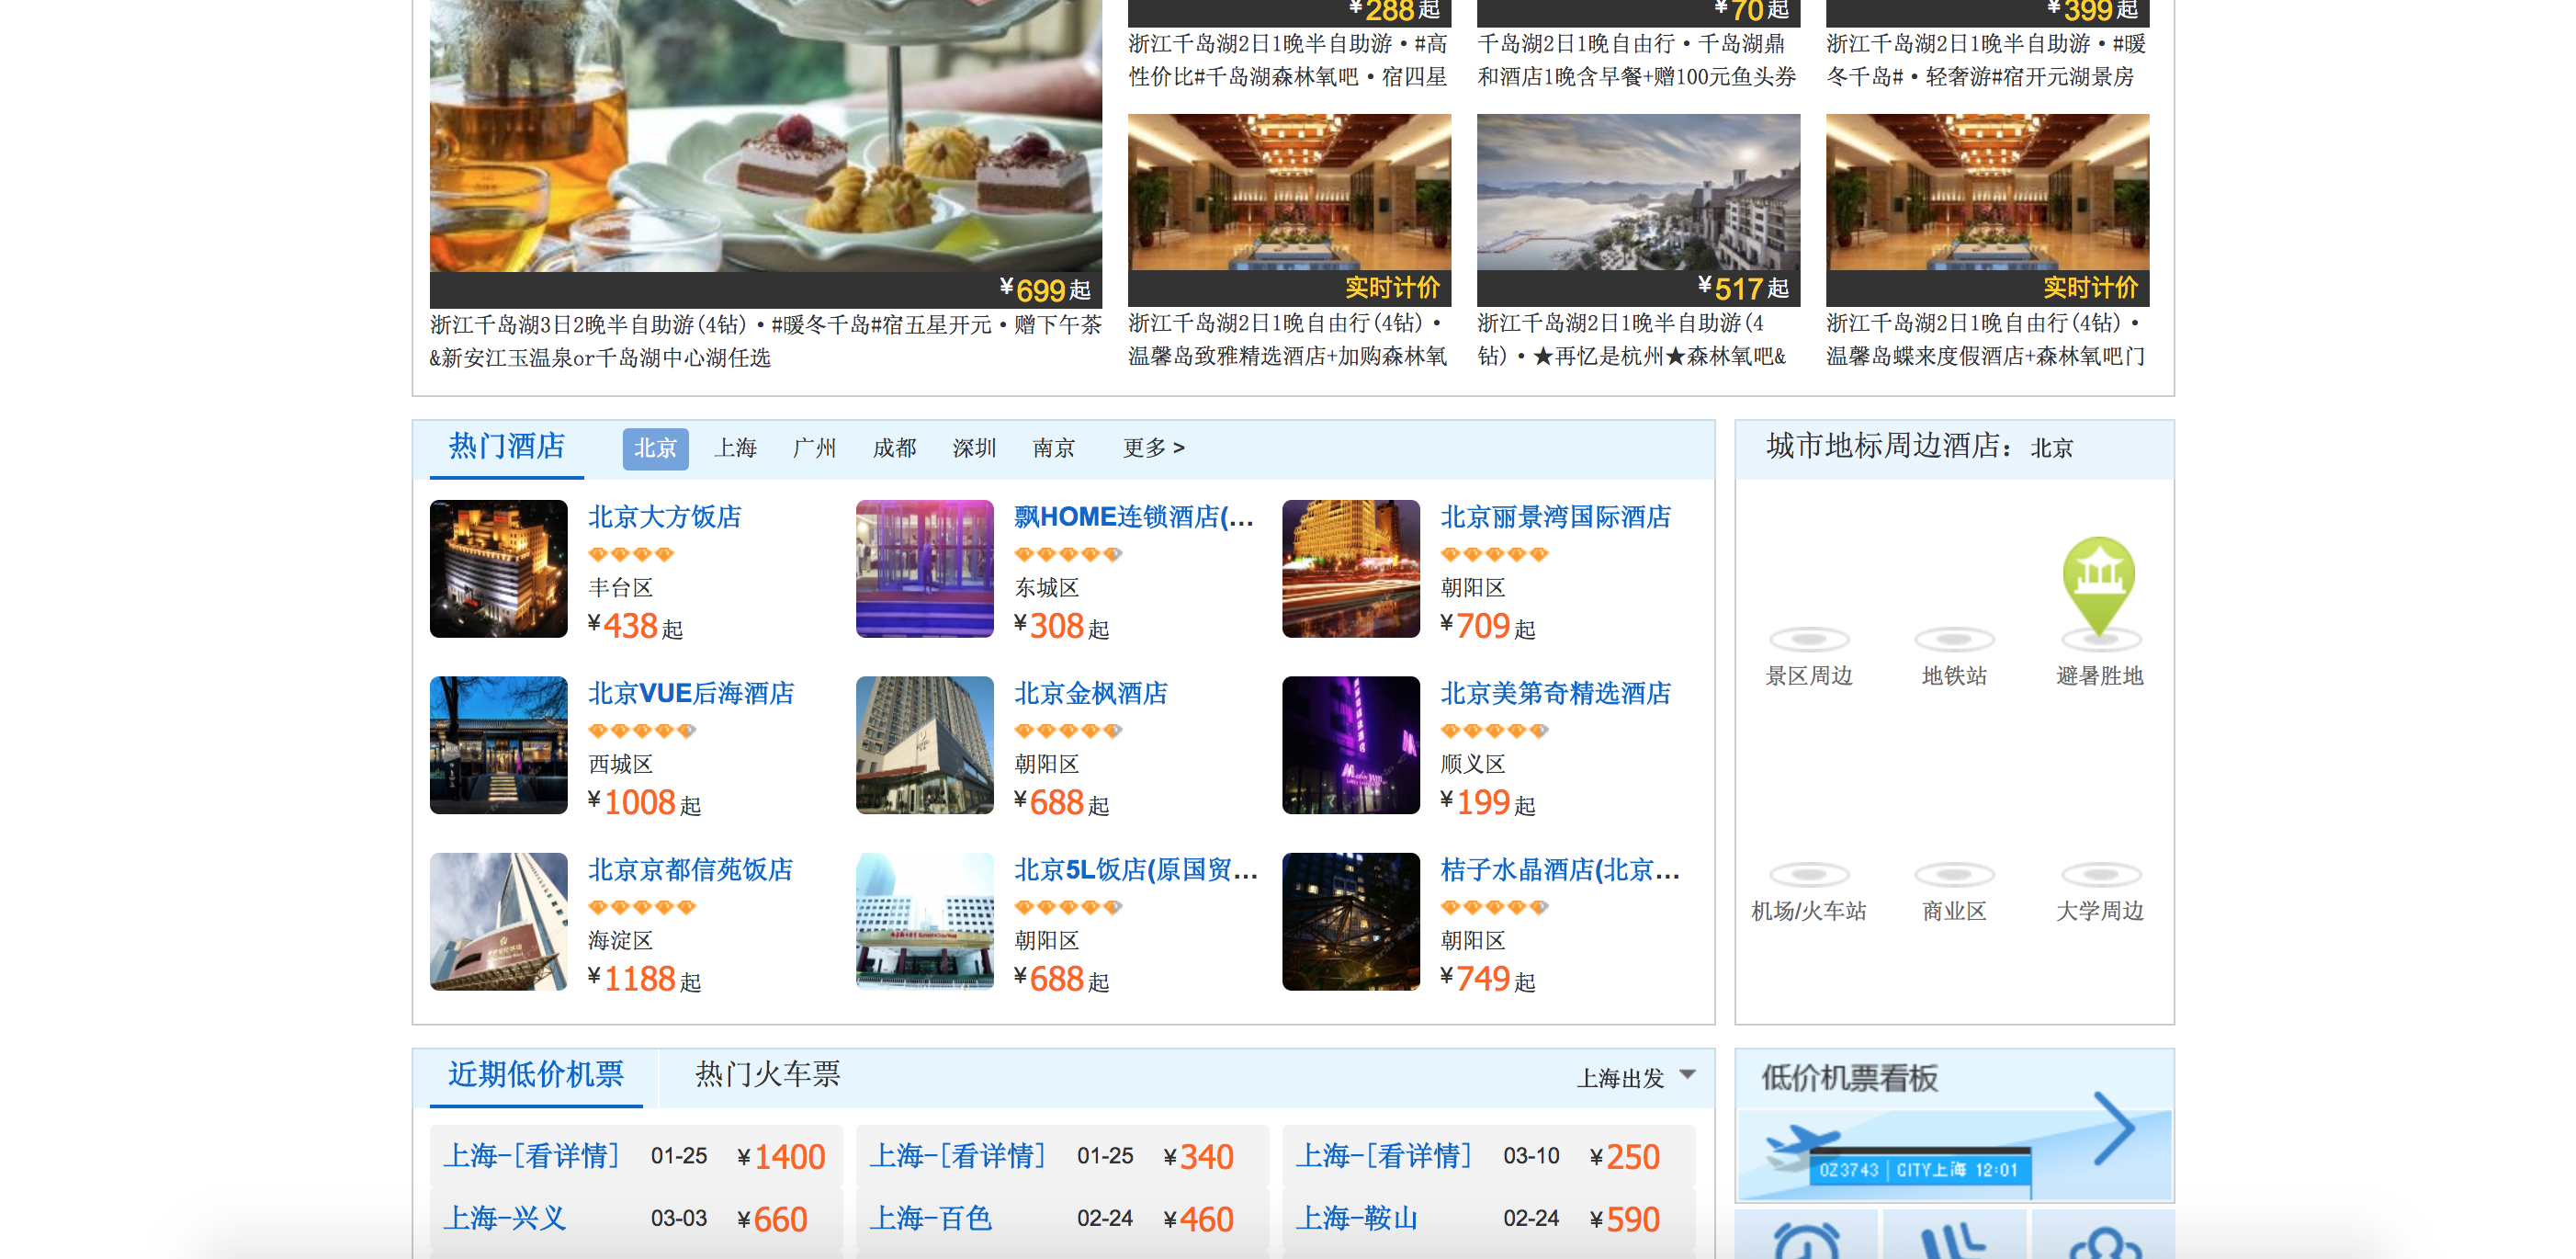
\includegraphics[width=100mm]{Images/ctrip_chinese2}
\decoRule
\caption[Chinese version of Ctrip]{The Chinese version of the travel website Ctrip.}
\label{fig:ctrip_chinese}
\end{figure}

\begin{figure}[h]
\centering
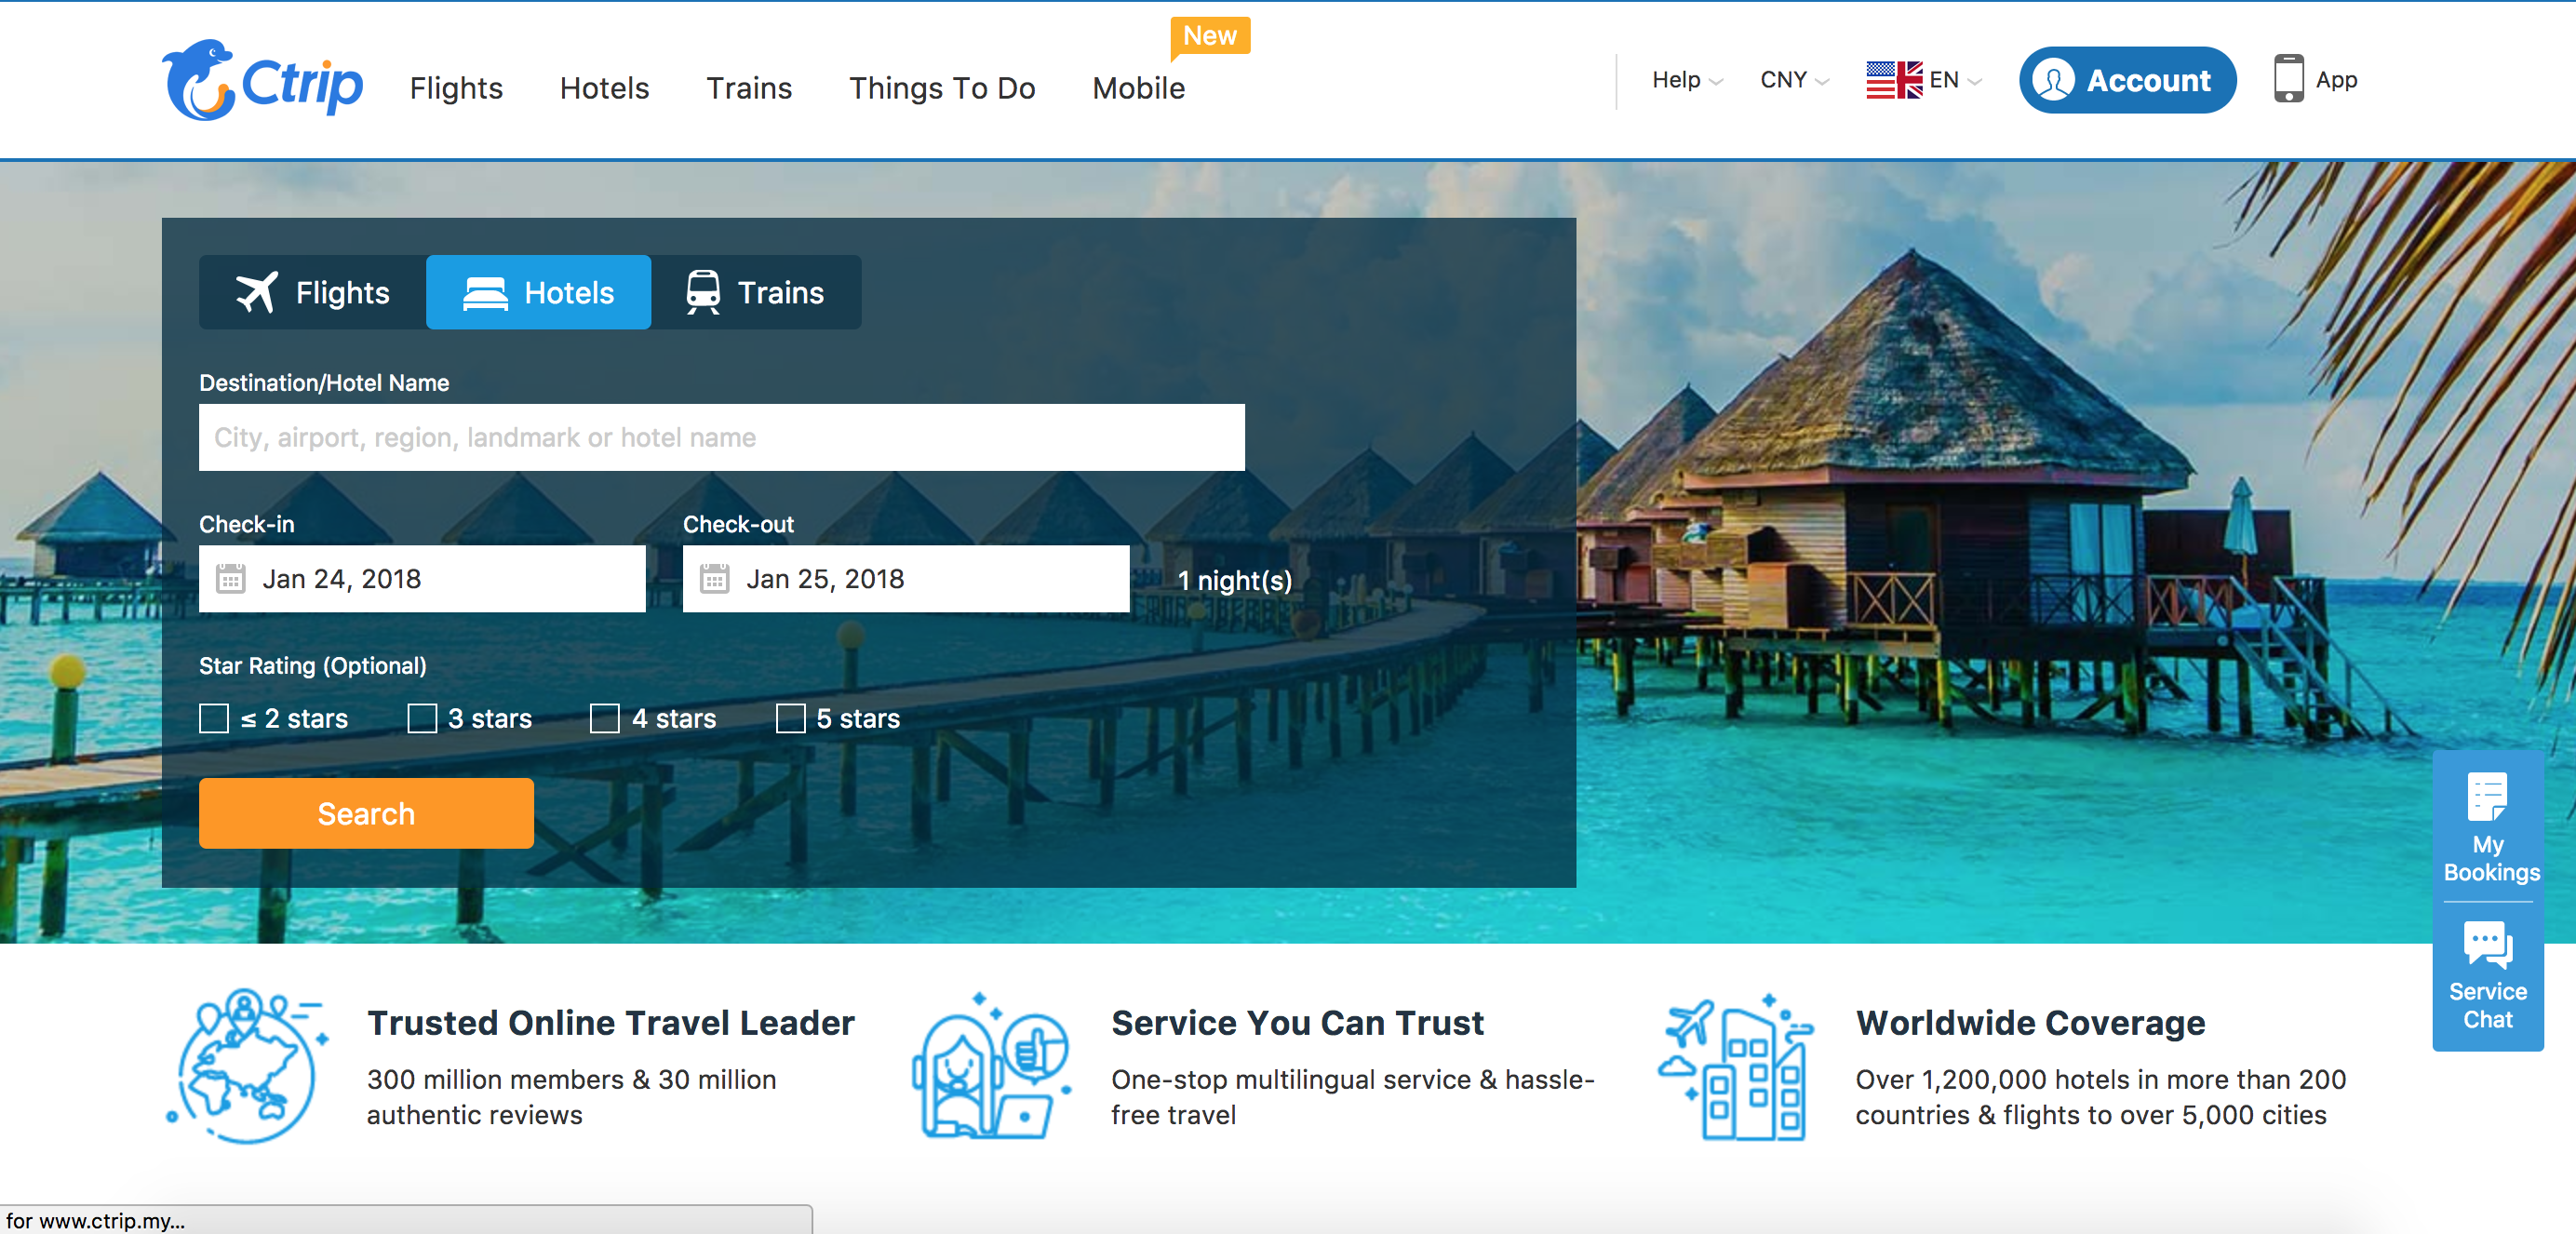
\includegraphics[width=100mm]{Images/ctrip_eng1}
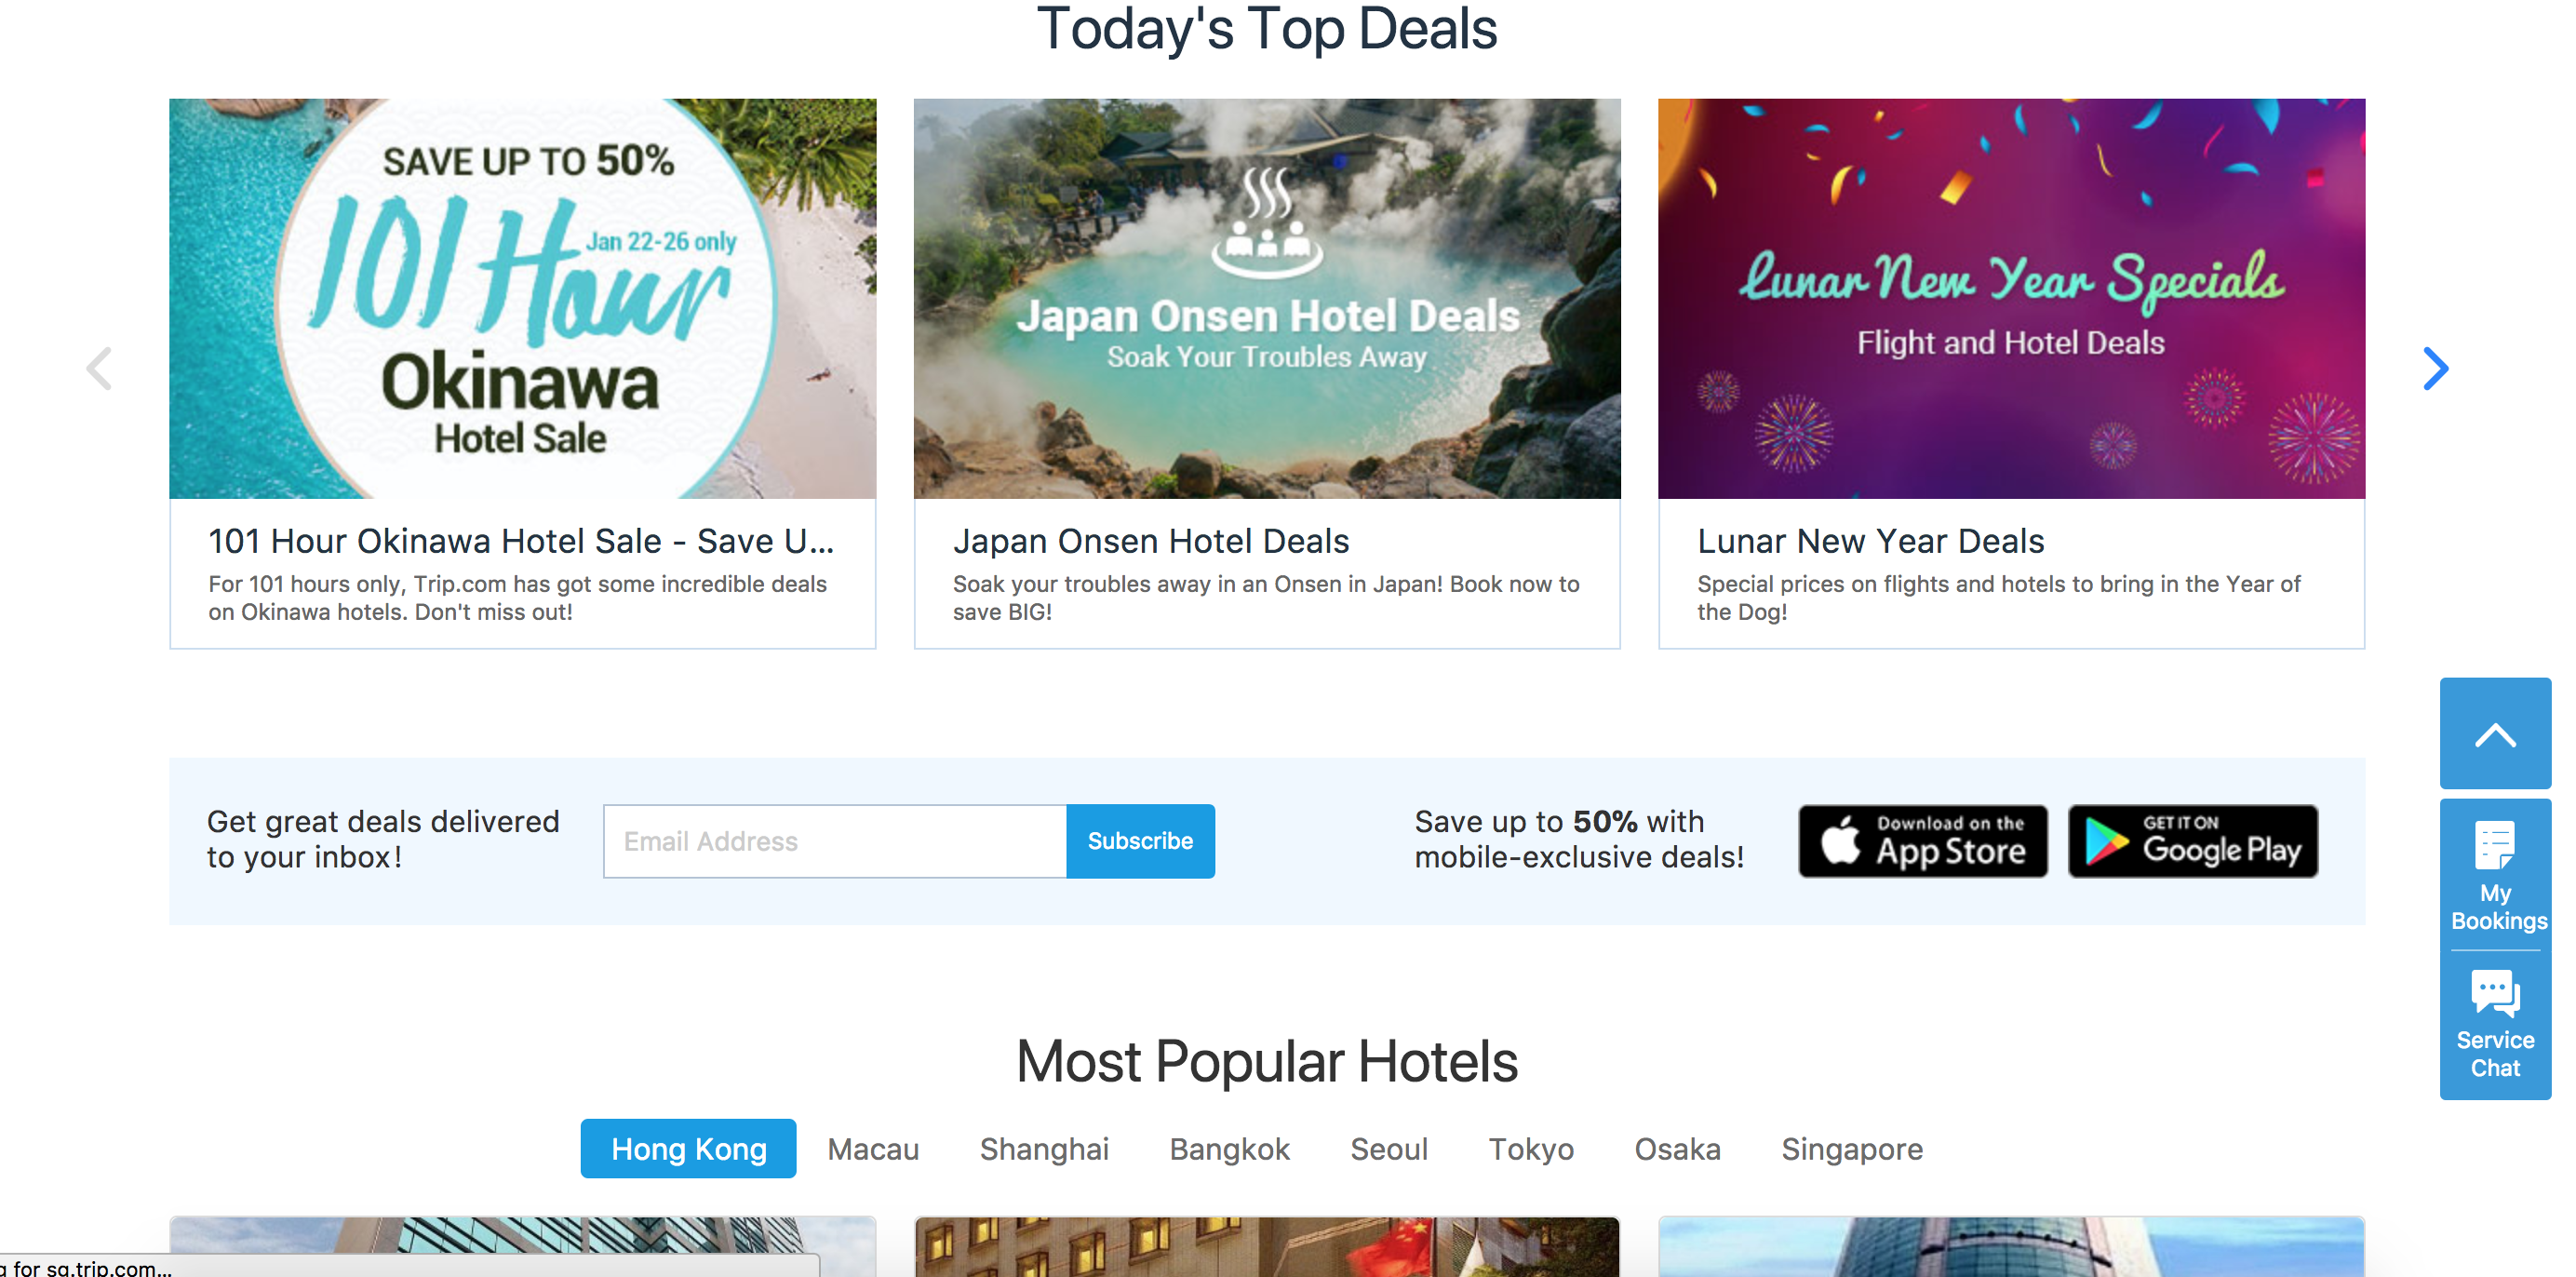
\includegraphics[width=100mm]{Images/ctrip_eng2}
\decoRule
\caption[English version of Ctrip]{The English version of the travel website Ctrip.}
\label{fig:ctrip_english}
\end{figure}
 The main difference documented between the sites is content density. The Chinese version of Ctrip has a lot more content in a small area compared to the English-translated version of the site. Counting clickable elements without hovering over anything, 40 clickable elements were found on the Chinese version compared to only 26 clickable elements on the English version. When using the Chinese site, all links open a separate window instead of a second menu or tab - a common phenomena found on Chinese sites.
 
 
 \section{Analysis}
Looking through the websites we can identify several design features (outside of the language differences) that differ in Chinese and western websites. 
\\\\
These are:
 \begin{itemize}
 \item High information density
 \item Colors
 \item Ad content
 \item Navigation
 \end{itemize}
 
 The main factor of variance across the sites is information density. Chinese websites have significantly higher information density compared to their western counterparts. As such, information density is one feature that will be closely examined in this research. Colors and navigation features will be explored, but not prioritized. These aforementioned features will be included to aid in understanding the look and feel of the sites, rather than being the primary objectives of investigation. Additionally, since Chinese sites contain a higher ratio of ad content compared to western sites. There are several theories accounting for why Chinese sites are more information dense. Some of these hypotheses are: cultural/trends, historical, holistic vs analytic perceptions and language. Due to limitations concerning Chinese language and knowledge of the history and culture, we will mainly examine trends and perception.
 \\\\
For the purposes of this research, different interfaces were created for the purpose of investigating trends and perception differences between sites. One page is western inspired and another was created with inspiration from Chinese designs. To ensure that the interfaces maintain authentic Chinese and western designs, professional UX-designers from Sweden and China assited in the development of some prototypes. These prototypes were then tested on both users with Swedish and Chinese heritages respectively. Finally, working interfaces, cable of measuring what actions users take in responding to certain tasks, was developed given the feedback from these prototypes. Main measurements that will be used are task-success, time-on-task and a modified System usability scale. \cite{brooke1996sus} 
 \\\\
 Four interfaces will be created, with two following a western design and the other two using a Chinese layout. The first interface takes inspiration from the QQ and BBC news site home pages. The goal of implementing these interfaces is to explore how fluidly users from different cultural backgrounds can navigate sites containing high information density (e.g., copious amounts of images and texts ). Both interfaces contain roughly equivalent levels of material and clickable elements; the primary difference is that the western site will be longer, forcing users to scroll down the page. Additionally, some of the information will be mapped in sub-menus using natural mapping for the western site \cite{Norman}. Conversely, the Chinese inspired site will provide most of the material directly on the screen for users to view without any nested menus. 

  

 \subsection{Work based on analysis}
  Choosing the ux questions:
  In \cite{Holistic_vs_Analytic} has shown that perception differs in western and eastern cultures. \cite{cross_web} further indicates that this perception difference holds true in the case of people observing websites. Specifically, users using analytical processing follow the F-shaped pattern when browsing sites \cite{pernice2014people}. Holistic thinkers, conversely, do not follow the F-shaped pattern when browsing through a website. \cite{cross_web} In light of these past studies, it will be interesting to explore how these perception differences will influence users' abilities to navigate and perceive web pages. To investigate this question, we select elements both in accordance to the F-shaped pattern and elements outside of this pattern. By testing the performance on both analytical and holistic thinkers, we should get an indication of the differences and  how well people follow the F-shaped pattern when looking for specific elements. The test will be unsupervised, meaning that we will have to get a larger test audience in order to obtain significant results. To test variances in perception, we will create tests for the sites BBC and QQ. On these pages, we will ask test subjects to find elements following an F-shaped pattern and elements not following this pattern.
   
 